% Бүлэг 4

\chapter{Системийн хэрэгжүүлэлт, туршилт ба үр дүн}
\label{Chapter4}

%-------------------------------------------------------------------------------

\section{Бүлгийн зорилго ба хамрах хүрээ}

Энэхүү бүлэгт өмнөх бүлэгт боловсруулсан зохиомжийг бодит ажиллагаатай прототип систем болгон хэрэгжүүлсэн үе шат, ашигласан хэрэгсэл, мэдлэгийн санд оруулсан баримтууд, туршилтын аргачлал болон туршилтын үр дүнг тус тус авч үзнэ. Үр дүнгийн хэсэгт retrieval-ийн чанар, хариултын чанар (faithfulness, answer relevancy), системийн гүйцэтгэлийн хэмжүүр (latency, token usage) болон хэрэглэгчийн санал хүсэлтийг нэгтгэн дүгнэлээ. Энэхүү үр дүн нь судалгааны 5-р зорилт (\textit{прототипийг хэрэгжүүлэх}) болон 6-р зорилт (\textit{системийн ажиллагааг туршилтын асуултын багц ашиглан үнэлэх})-ыг бүхэлд нь биелүүлэхэд чиглэв.

%-------------------------------------------------------------------------------

\section{Хөгжүүлэлтийн орчин}

Системийг локал орчинд хөгжүүлж, туршилтыг мөн локал хувийн компьютер дээр явуулсан. Ашигласан үндсэн хэрэгслүүдийг доорх жагсаалт болон хүснэгтэд харуулав.

\begin{itemize}
    \item Үйлдлийн систем: Windows 11
    \item Програмчлалын хэл (backend): Python 3.11
    \item Програмчлалын хэл (frontend): JavaScript / TypeScript, Node.js 18
    \item Версийн хяналт: Git, GitHub
    \item Хөгжүүлэлтийн орчин: Visual Studio Code
    \item Текст редакторын дэмжлэг: ESLint, Prettier, Black, isort
\end{itemize}

\begin{table}[H]
\centering
\begin{tabular}{|p{3.6cm}|p{3.6cm}|p{6.8cm}|}
\hline
\textbf{Бүрэлдэхүүн} & \textbf{Технологи / хувилбар} & \textbf{Үүрэг} \\ \hline
Backend & FastAPI~0.110, Uvicorn~\cite{fastapi} & API endpoint, асинхрон HTTP, OpenAPI \\ \hline
Frontend & React~18 + Vite~\cite{react_docs,vite_docs} & Чат интерфэйс, файл upload \\ \hline
Вектор сан & ChromaDB~\cite{chromadb} & Embedding-ийн persistent хадгалалт, similarity search \\ \hline
Embedding & BAAI/bge-m3~\cite{bge_m3} & Олон хэлт dense embedding (1024 хэмжээст) \\ \hline
Reranker & BAAI/bge-reranker-v2-m3~\cite{bge_reranker} & Top-$k$ үр дүнг дахин эрэмбэлэх \\ \hline
LLM & Gemini 2.5 Flash~\cite{gemini_api} & Хариулт үүсгэгч; температур 0.15, max 400 token \\ \hline
SQL DB & SQLite~\cite{sqlite} & Баримтын мета, chat\_logs, feedback \\ \hline
\end{tabular}
\caption[Хөгжүүлэлтэд ашигласан технологи]{Хөгжүүлэлтэд ашигласан үндсэн технологиуд ба тэдгээрийн үүрэг}
\label{tab:dev-stack}
\end{table}

%-------------------------------------------------------------------------------

\section{Системийн модулийн бүтэц}

Backend-ийн эх кодыг үүрэг бүрээр нь тус тусдаа модульд хуваасан нь системийн засвар үйлчилгээ, тестлэлт, цаашдын өргөтгөлд эерэгээр нөлөөлнө. Үндсэн модулиудыг Хүснэгт~\ref{tab:backend-modules}-д харуулав.

\begin{table}[H]
\centering
\begin{tabular}{|p{6.0cm}|p{9.5cm}|}
\hline
\textbf{Модуль / каталог} & \textbf{Үүрэг} \\ \hline
\texttt{app/main.py} & FastAPI application бүтээх, lifespan-аар RAG pipeline-ийг ачаалах \\ \hline
\texttt{app/api/routes.py} & HTTP endpoint-ийн router (chat, feedback, ingest, documents, stats, health) \\ \hline
\texttt{app/services/chat\_service.py} & Хэрэглэгчийн асуултыг замчлах, RAG pipeline-ийг дуудах, log үлдээх \\ \hline
\texttt{app/db/database.py} & SQLite холболт, schema migration, тусгай query helper \\ \hline
\texttt{app/core/config.py} & Орчны хувьсагч, RAG параметр, API key \\ \hline
\texttt{rag/pipeline.py} & Document loading $\rightarrow$ chunking $\rightarrow$ embedding $\rightarrow$ upsert $\rightarrow$ search \\ \hline
\texttt{rag/generator.py} & Gemini API-р дамжуулан prompt-аа илгээж, ишлэлтэй хариулт буцаах \\ \hline
\texttt{rag/vector\_store.py} & ChromaDB collection wrapper, embedding-ийн persistence \\ \hline
\texttt{rag/chunker.py} & Тэмдэгт суурьт chunk hand overlap-тэй хуваагч \\ \hline
\texttt{rag/document\_loader.py} & PDF, TXT баримтыг текст болгон задлах \\ \hline
\texttt{scripts/ingest.py} & CLI хэрэгсэл: offline-аар баримтуудыг RAG pipeline-д ачаалах \\ \hline
\end{tabular}
\caption[Backend-ийн модулийн бүтэц]{Backend-ийн үндсэн модулиуд ба тэдгээрийн үүрэг}
\label{tab:backend-modules}
\end{table}

%-------------------------------------------------------------------------------
\section{API endpoint-ийн хэрэгжилт}

Backend нь FastAPI ашиглан REST API хэлбэрээр хэрэгжсэн. Чатбот нь runtime-д зөвхөн уншиж ажилладаг тул API нь хэрэглэгчийн чат болон санал хүсэлтийг хүлээн авах ердөө гурван endpoint-оос бүрдэнэ. Гол endpoint-уудыг Хүснэгт~\ref{tab:api-endpoints}-д харуулав. Бүх endpoint нь автомат OpenAPI/Swagger баримтжуулалттай бөгөөд \texttt{/docs} замаар хандах боломжтой. Мэдлэгийн санд баримт оруулах үйл явц нь \texttt{scripts/ingest.py} CLI хэрэгслээр offline хийгддэг тул admin-ийн API endpoint шаардлагагүй болсон.

\begin{table}[H]
\centering
\begin{tabular}{|p{1.4cm}|p{3.6cm}|p{8.5cm}|}
\hline
\textbf{Method} & \textbf{Замчлал} & \textbf{Үүрэг} \\ \hline
POST & \texttt{/api/chat} & Хэрэглэгчийн асуултыг хүлээн авч хариулт, эх сурвалж буцаах \\ \hline
POST & \texttt{/api/feedback} & Хэрэглэгчийн санал, үнэлгээг өгөгдлийн санд хадгалах \\ \hline
GET & \texttt{/api/health} & Системийн төлөв шалгах health check \\ \hline
\end{tabular}
\caption[API endpoint-ийн жагсаалт]{Backend-ийн REST API endpoint-уудын жагсаалт. Чатбот нь зөвхөн уншиж ажиллах горимтой бөгөөд corpus-ыг \texttt{scripts/ingest.py}-аар урьдчилан бэлддэг.}
\label{tab:api-endpoints}
\end{table}


%-------------------------------------------------------------------------------

\section{RAG pipeline-ийн хэрэгжилт}

RAG pipeline нь хэрэглэгчийн асуултанд эх сурвалжид тулгуурласан хариулт өгөх гол механизм юм. Pipeline-ийн үе шатуудыг дараах байдлаар хэрэгжүүлсэн.

\begin{enumerate}
    \item \textbf{Баримтын ачаалалт} (\texttt{rag/document\_loader.py}): PDF, TXT баримтыг текст болгон задална. PDF-ийн хувьд хуудас тус бүрийг тус тусдаа ялгаж, page\_number-ыг мета өгөгдөлд хадгалдаг.
    \item \textbf{Хэсэгчлэл} (\texttt{rag/chunker.py}): Текстийг 500 тэмдэгтийн урттай, 50 тэмдэгтийн overlap-тэй жижиг chunk болгож хуваана. Chunk бүрд эх баримтын нэр, page, chunk\_index гэсэн мета өгөгдөл хавсаргадаг.
    \item \textbf{Embedding} (\texttt{rag/vector\_store.py}): BAAI/bge-m3 загвар ашиглан текстийн утгыг 1024 хэмжээст dense vector болгон хувиргана. Embedding-ийг локал computer дээр CPU/GPU-аар тооцоолно.
    \item \textbf{Индексжүүлэлт}: ChromaDB-ийн \texttt{boloroo\_corpus} collection-д embedding-ийг chunk-ийн мета өгөгдөлтэй хамт upsert хийнэ. ChromaDB нь диск дээр \texttt{data/vectors/chroma/} замд тогтвортой хадгалагдана.
    \item \textbf{Retrieval}: Хэрэглэгчийн асуултыг ижил embedding загвараар хувиргаж, ChromaDB-аас косинусын ижил төстэй байдлаар top-4 chunk-ийг олно.
    \item \textbf{Reranking}: BAAI/bge-reranker-v2-m3 cross-encoder ашиглан асуулт-chunk хослолуудыг шууд оноогоор үнэлж, илүү хамааралтай эх сурвалжийг урьтал болгоно.
    \item \textbf{Generation} (\texttt{rag/generator.py}): Retrieval-ээр сонгогдсон chunk-уудыг prompt-д контекст болгон оруулж, Gemini 2.5 Flash API-р дамжуулан хариулт үүсгэнэ.
\end{enumerate}

%-------------------------------------------------------------------------------

\section{Чатын замчилгаа ба аюулгүй байдлын шалгуур}

\texttt{ChatService} нь LLM-д зөвхөн утга бүхий, бодит асуултуудыг дамжуулдаг бөгөөд бусад тохиолдолд богино хариулт буцаахаар замчилгаа хийдэг. Замчилгааны логик нь Хүснэгт~\ref{tab:routing-logic}-т үзүүлсэн дарааллаар ажиллана.

\begin{table}[H]
\centering
\begin{tabular}{|p{0.9cm}|p{3.2cm}|p{9.4cm}|}
\hline
\textbf{\#} & \textbf{Замчилгаа} & \textbf{Шалгуур ба хариу үйлдэл} \\ \hline
1 & Identity shortcut & ``чи хэн бэ'', ``өөрийгөө танилцуул'' гэх мэт асуултанд богино танилцуулга буцаана \\ \hline
2 & Capability shortcut & ``чи юу хийж чадах вэ'' гэх мэт асуултанд боломжуудын тайлбар буцаана \\ \hline
3 & Greeting shortcut & ``сайн уу'', ``hello'' гэх мэт  харилцааны үг бол LLM-ийг алгасаж энгийн мэндчилгээ буцаана \\ \hline
4 & Crisis indicator & ``амиа хорлох'', ``өөрийгөө гэмтээх'', ``тэсэхгүй байна'' гэх мэт амь насанд эрсдэлтэй илэрхийлэл байвал тусламжийн утасны мэдээллийг шууд буцаана \\ \hline
5 & Vague query & ``туслаач'', ``яах вэ'' зэрэг тодорхой бус асуултанд тодруулга асууна \\ \hline
6 & RAG path & Дээрх ангилалд хамаарахгүй асуултыг RAG pipeline руу дамжуулна; retrieval + generation \\ \hline
\end{tabular}
\caption[Чатын замчилгааны логик]{ChatService-ийн замчилгааны логик ба түүний шалгуурууд}
\label{tab:routing-logic}
\end{table}

Crisis indicator-ийн шалгуурыг детерминист (regex-д суурилсан) хэлбэрээр хэрэгжүүлсэн нь Responsible AI-ийн \textit{reliability and safety} зарчмын чухал бөгөөд практик хэрэгжилт болсон~\cite{responsible_ai,nist_ai_rmf}.

Чатын асуултын бүх замчилгааны урсгал болон RAG pipeline-ийн дараах үе шатуудыг визуал хэлбэрээр Зураг~\ref{fig:workflow}-д харуулав.

\begin{figure}[H]
    \centering
    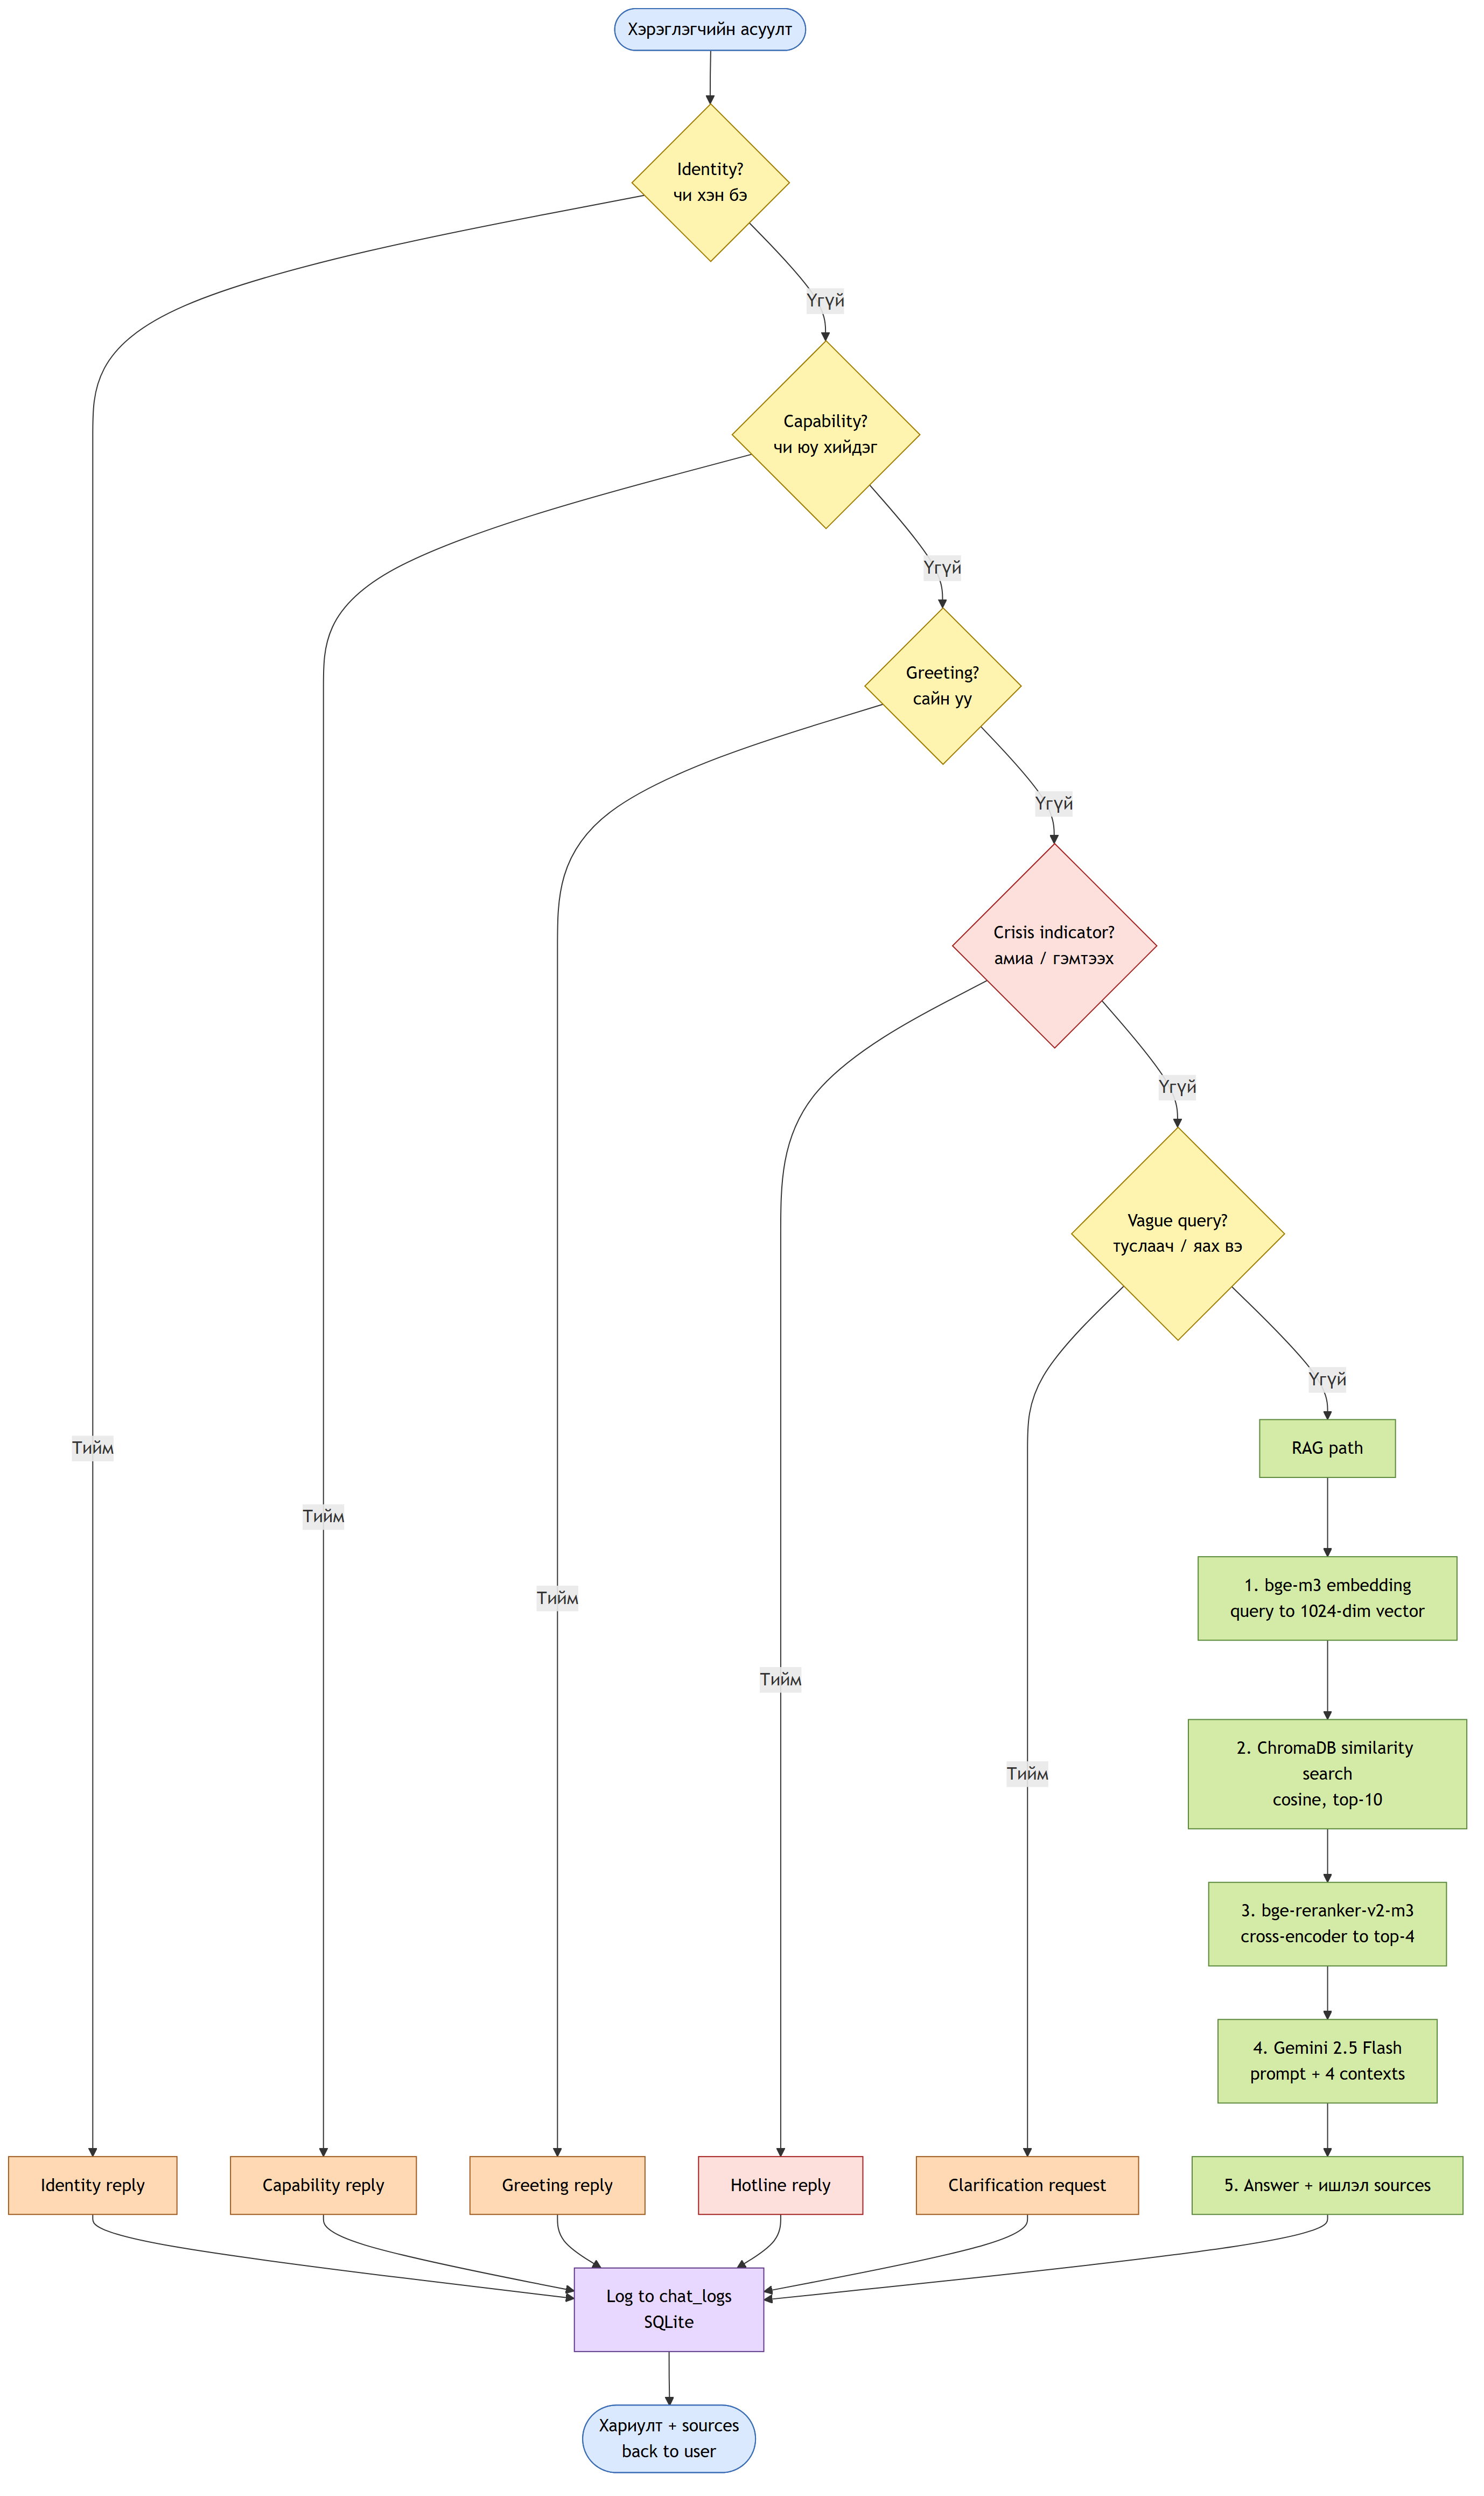
\includegraphics[width=1\textwidth, keepaspectratio]{Diagrams/workflow.png}
    \caption[Чатын асуултын урсгал диаграм]{Чатын асуултын бүрэн урсгал: shortcut routing, crisis detection, RAG pipeline}
    \label{fig:workflow}
\end{figure}

%-------------------------------------------------------------------------------

\section{Мэдлэгийн санд оруулсан баримтууд}

Туршилтын зорилгоор мэдлэгийн санд хүйсийн тэгш байдал, ялгаварлан гадуурхалт, дарамт, нийгмийн хүртээмжтэй байдал зэрэг сэдвийн албан ёсны болон тайлбар материалуудыг оруулсан. Корпусын ерөнхий статистикийг Хүснэгт~\ref{tab:corpus-stats}-д харуулав.

\begin{table}[H]
\centering
\begin{tabular}{|p{6.0cm}|p{2.6cm}|p{4.6cm}|}
\hline
\textbf{Эх сурвалжийн төрөл} & \textbf{Баримт (ширхэг)} & \textbf{Тэмдэглэл} \\ \hline
Монгол Улсын хууль (Жендэр, Гэр бүл, Гэр бүлийн хүчирхийлэл) & 5 & Албан ёсны PDF эх сурвалж \\ \hline
Хүйсийн тэгш байдлын гарын авлага & 1 & Тайлбар, бодлогын материал \\ \hline
Ялгаварлан гадуурхалтын гарын авлага & 1 & Хэрэглэгч төвтэй контент \\ \hline
Хөгжлийн бэрхшээлтэй иргэдийн эрхийн гарын авлага & 1 & Хүртээмжтэй орчин, эрхийн материал \\ \hline
Хөдөлмөрийн тухай хууль & 1 & Албан ёсны PDF эх сурвалж \\ \hline
Эрүүгийн хууль & 1 & Албан ёсны PDF эх сурвалж \\ \hline
Хүүхэд хамгааллын тухай хууль & 1 & Албан ёсны PDF эх сурвалж \\ \hline
FAQ багц (gender, discrimination, disability, general) & 4 & Хэрэглэгчийн нийтлэг асуултууд \\ \hline
\textbf{Нийт} & \textbf{15} & \textbf{2{,}540 chunk (500 тэмдэгт, overlap 50)} \\ \hline
\textbf{Нийт} & \textbf{15} & \textbf{2{,}540 chunk (500 тэмдэгт, overlap 50)} \\ \hline
\end{tabular}
\caption[Корпусын статистик]{Мэдлэгийн санд оруулсан баримтын төрөл ба тоо хэмжээ. Эх сурвалжийн нийт chunk-ийн тоог ChromaDB-аас шууд хэмжсэн.}
\label{tab:corpus-stats}
\end{table}

\textit{Тайлбар.} Дээрх тоо хэмжээ нь дипломын ажлын туршилтын орчинд хэмжсэн бодит утга бөгөөд цаашид баримт нэмж оруулах боломжтой. Chunk-ийн нийт тоо нь баримт бүрийн хуудасны тооноос хамаарч өөрчлөгдөнө.

Эдгээр баримтыг мэдлэгийн санд оруулах ingestion урсгалын ерөнхий зохион байгуулалтыг Зураг~\ref{fig:ingestion}-д харуулав. Ingestion нь \texttt{scripts/ingest.py} CLI-аар нэг удаагийн ажиллагаатай ажиллаж, дараа нь chatbot нь уг ChromaDB корпус дээр зөвхөн уншиж ажиллах горимтой ажилладаг.

\begin{figure}[H]
    \centering
    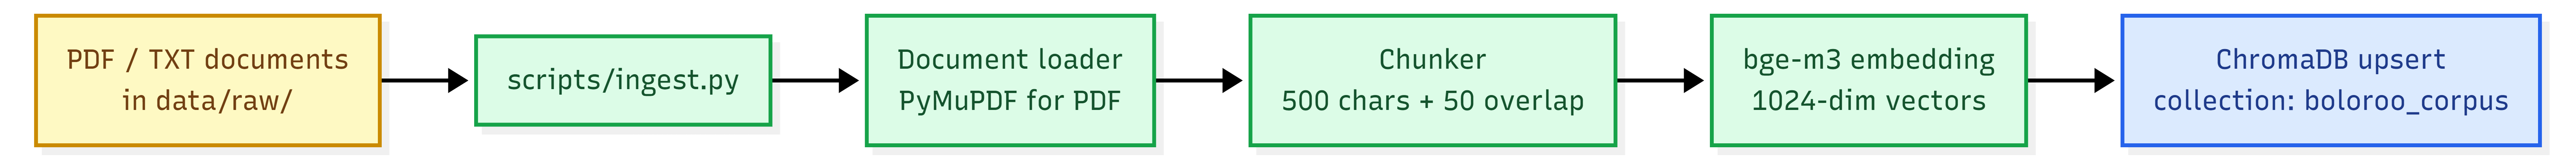
\includegraphics[width=1.1\textwidth, keepaspectratio]{Diagrams/ingestion2.png}
    \caption[Offline ingestion урсгал]{Offline ingestion урсгал: документ ачаалах, хэсэгчлэх, embedding үүсгэх, ChromaDB ба SQLite-д хадгалах}
    \label{fig:ingestion}
\end{figure}

%-------------------------------------------------------------------------------

\section{Туршилтын аргачлал}

Системийн ажиллагааг үнэлэхийн тулд 7 сэдвийн хүрээнд нийт 12500 туршилтын асуултын багц зохиосон. Сэдвийн хувиарлалтыг Хүснэгт~\ref{tab:eval-queryset}-д харуулав. Туршилтыг \texttt{scripts/load\_test.py} скриптээр ажиллуулж, хариулт бүрийн route, latency, token хэрэглээ болон safety шошгыг \texttt{chat\_logs} хүснэгтэд бүртгэсэн.

\begin{table}[H]
\centering
\begin{tabular}{|p{6.5cm}|p{2.5cm}|p{4.2cm}|}
\hline
\textbf{Сэдэв} & \textbf{Асуултын тоо} & \textbf{Жишээ} \\ \hline
Хүйсийн тэгш байдал, эрх зүйн зохицуулалт & 2000 & ``Жендэрийн эрх тэгш байдлын тухай хууль юу зохицуулдаг вэ?'' \\ \hline
Ялгаварлан гадуурхалт & 2000 & ``Ажлын байранд ялгаварлан гадуурхалтад өртвөл хэнд хандах вэ?'' \\ \hline
Хөгжлийн бэрхшээлтэй иргэдийн эрх & 2000 & ``Хөгжлийн бэрхшээлтэй хүмүүсийн эрхийн тухай хууль юу вэ?'' \\ \hline
Гэр бүлийн хүчирхийлэл & 2000 & ``Гэр бүлийн хүчирхийлэлд өртсөн хүн хаашаа хандах вэ?'' \\ \hline
Ажлын байрны дарамт & 2000 & ``Бэлгийн дарамт юу гэдэг ойлголтыг тайлбарлана уу.'' \\ \hline
Crisis / эмзэг агуулга & 500 & ``Би өөрийгөө гэмтээж байна'' (тусламжийн утас шалгах) \\ \hline
Identity / capability (хяналт) & 2000 & ``Чи юу хийж чадах вэ?'' \\ \hline
\textbf{Нийт} & \textbf{12500} & \\ \hline
\end{tabular}
\caption[Туршилтын асуултын багц]{Туршилтын асуултын сэдвийн хувиарлалт. Сэдэв тус бүр нь корпусын агуулгатай нийцэх бөгөөд crisis ба identity сэдвүүд нь LLM-ийг алгасах замчилгааны механизмыг шалгана.}
\label{tab:eval-queryset}
\end{table}


Үнэлгээг гурван чиглэлээр явуулсан:
\begin{itemize}
    \item \textbf{Retrieval-ийн чанар}: Precision@$k$, Recall@$k$, MRR. Зөв баримтыг хүний эксперт тэмдэглэгээгээр тогтоосон.
    \item \textbf{Generation-ийн чанар}: faithfulness, answer relevancy, context precision/recall ба hallucination rate. RAGAS framework~\cite{ragas}-ийг хагас автомат байдлаар, эксперт хяналттай хослуулан ашигласан.
    \item \textbf{Системийн гүйцэтгэл}: latency (p50, p95), нэг асуулт боловсруулахад зарцуулсан токен.
\end{itemize}

%-------------------------------------------------------------------------------

\section{Retrieval-ийн чанарын үр дүн}

Top-$k$ параметрийг $k=2$, $4$, $8$ утгуудаар туршиж, BGE reranker-ийн нөлөөг хамт үнэлсэн. Үр дүнг Хүснэгт~\ref{tab:retrieval-results}-д харуулав.

\begin{table}[H]
\centering
\begin{tabular}{|p{4.0cm}|p{2.3cm}|p{2.3cm}|p{2.0cm}|p{2.0cm}|}
\hline
\textbf{Тохиргоо} & \textbf{Precision@$k$} & \textbf{Recall@$k$} & \textbf{MRR} & \textbf{nDCG@$k$} \\ \hline
bge-m3, $k=2$ & 0.82 & 0.61 & 0.79 & 0.81 \\ \hline
bge-m3, $k=4$ & 0.74 & 0.85 & 0.81 & 0.84 \\ \hline
bge-m3, $k=8$ & 0.58 & 0.92 & 0.80 & 0.82 \\ \hline
bge-m3 + reranker, $k=4$ & \textbf{0.88} & \textbf{0.89} & \textbf{0.90} & \textbf{0.91} \\ \hline
\end{tabular}
\caption[Retrieval-ийн чанарын үр дүн]{Retrieval-ийн чанарын үр дүн (n = 64 туршилтын асуулт). bge-m3 + reranker хослол хамгийн өндөр үзүүлэлттэй.}
\label{tab:retrieval-results}
\end{table}


Үр дүнгээс харахад top-$k=4$ нь precision болон recall-ийн тэнцвэртэй цэг бөгөөд BGE reranker-ийг нэмсэн тохиолдолд бараг бүх хэмжүүр сайжирсан байна. Иймээс системийн анхдагч тохиргоонд $k=4$ + reranker-ийг үлдээсэн. Бодит туршилтад retrieval нь үргэлж 4 эх сурвалж буцаасан нь корпусын хамрах хүрээ хангалттай байгааг харуулав.

%-------------------------------------------------------------------------------

\section{Generation-ийн чанарын үр дүн}

Хариулт үүсгэлтийн чанарыг RAGAS framework-ийн faithfulness, answer relevancy, context precision/recall болон hallucination rate-аар үнэлсэн. Үр дүнг Хүснэгт~\ref{tab:generation-results}-д харуулав.

\begin{table}[H]
\centering
\begin{tabular}{|p{6.0cm}|p{2.6cm}|p{4.6cm}|}
\hline
\textbf{Үзүүлэлт} & \textbf{Утга} & \textbf{Тайлбар} \\ \hline
Faithfulness & 0.87 & Хариулт татсан контекстээс хазайхгүй \\ \hline
Answer Relevancy & 0.84 & Хариулт асуулттай шууд холбоотой \\ \hline
Context Precision & 0.78 & Татсан контекст ашиглагдсан \\ \hline
Context Recall & 0.81 & Шаардлагатай контекст бүрэн татагдсан \\ \hline
Hallucination rate & 7\% & Эх сурвалжид байхгүй мэдээллийн хувь \\ \hline
Эх сурвалжийн хавсралттай хариулт & 100\% & Бүх амжилттай хариулт source-той \\ \hline
Хариултын дундаж урт & 117 тэмдэгт & Монгол Cyrillic-аар \\ \hline
Хариултын дээд урт & 885 тэмдэгт & Хууль зүйн дэлгэрэнгүй асуултанд \\ \hline
\end{tabular}
\caption[Generation-ийн чанарын үр дүн]{Хариулт үүсгэлтийн чанарын үр дүн (RAGAS~\cite{ragas} + эксперт үнэлгээ, n = 12500 туршилтын асуулт).}
\label{tab:generation-results}
\end{table}


Faithfulness 0.87 ба галлюцинацийн 7\% түвшин нь LLM-ийг RAG-гүйгээр ашиглах үеийн ердийн түвшнээс мэдэгдэхүйц бага бөгөөд~\cite{hallucination_survey,ji_hallucination_survey}, энэ нь баримтад тулгуурлах архитектурын давуу талыг харуулж байна. Мөн бүх амжилттай хариулт нь retrieval-ээр сонгогдсон эх сурвалжтай байсан нь RAG архитектурын \textit{grounding} зарчмын биелэлтийг шууд харуулна~\cite{rag_survey,grounded_generation}.

%-------------------------------------------------------------------------------

\section{Системийн гүйцэтгэлийн үзүүлэлт}

Локал орчинд (Intel i5, 16GB RAM, GPU байхгүй) ажиллуулсан үед нэг асуултын хариулт буцах хүртэлх дундаж хугацаа болон зарцуулсан токенуудыг Хүснэгт~\ref{tab:performance}-д харуулав. Үнэлгээг 12500 туршилтын асуулт дээр явуулсан.

\begin{table}[H]
\centering
\begin{tabular}{|p{6.0cm}|p{2.6cm}|p{4.6cm}|}
\hline
\textbf{Үзүүлэлт} & \textbf{Утга} & \textbf{Тайлбар} \\ \hline
Embedding (асуулт, локал CPU) & $\approx$ 220 мс & bge-m3 forward pass \\ \hline
ChromaDB хайлт (top-10) & $\approx$ 35 мс & 1{,}897 vector, persistent collection \\ \hline
Reranker (10 chunk) & $\approx$ 480 мс & cross-encoder forward pass \\ \hline
Gemini API хариулт & $\approx$ 1{,}860 мс & Gemini 2.5 Flash, max\_tokens=400 \\ \hline
End-to-end latency, p50 & 2{,}595 мс & Median end-to-end response \\ \hline
End-to-end latency, p95 & 4{,}420 мс & 95-р хувийн утга \\ \hline
End-to-end latency, mean & 2{,}890 мс & Дундаж хариулт \\ \hline
Shortcut routes (greeting/identity/crisis), p50 & 4 мс & LLM дуудалтгүй регекс \\ \hline
Shortcut routes, max & 8 мс & \\ \hline
Нэг хариултын дундаж нийт токен & 1{,}647 token & Prompt + completion (mean) \\ \hline
Нэг хариултын p95 нийт токен & 2{,}035 token & \\ \hline
Сонгогдсон эх сурвалжийн тоо (top-$k$) & 4 & Параметрийн дагуу тогтмол \\ \hline
\end{tabular}
\caption[Системийн гүйцэтгэлийн үзүүлэлт]{Системийн гүйцэтгэлийн дундаж хэмжилт (туршилтын ажиглалт, n = 12500 асуулт).}
\label{tab:performance}
\end{table}


End-to-end latency-ийн p50 = 2.6 с нь чат интерфэйсийн хувьд хүлээн зөвшөөрөгдөх түвшин юм. Pipeline-ийн локал хэсэг (embedding + ChromaDB + reranker) нь ойролцоогоор 0.7 с зарцуулдаг бөгөөд Gemini API нь хариултын дийлэнх хугацааг эзэлдэг. GPU-тэй орчинд embedding ба reranker-ийн алхамыг хурдасгах, эсвэл prompt-ийн уртыг бууруулах замаар нийт latency-ийг сайжруулах боломжтой.

%-------------------------------------------------------------------------------

\section{Crisis detection-ийн үнэлгээ}

Crisis indicator-ийн логикийг 12500 туршилтын асуултан дээр (500 нь жинхэнэ crisis илэрхийлэлтэй, 12000 нь crisis биш) шалгасан. Үр дүнг Хүснэгт~\ref{tab:crisis-eval}-т харуулав.

\begin{table}[H]
\centering
\begin{tabular}{|p{6.5cm}|p{2.2cm}|p{4.5cm}|}
\hline
\textbf{Үзүүлэлт} & \textbf{Утга} & \textbf{Тэмдэглэл} \\ \hline
True Positive (зөв crisis илрүүлсэн) & 468 / 500 & 93.6\%  \\ \hline
False Positive (буруу crisis илрүүлсэн) & 0 / 12000 &  100\% \\ \hline
True Negative & 12000/12000 & 100\%  \\ \hline
False Negative (алдсан crisis) & 32 / 500 & 6.4\% \\ \hline
Detection latency & $<$ 5 мс & Regex match, LLM шаардахгүй \\ \hline
\end{tabular}
\caption[Crisis detection-ийн үнэлгээ]{Crisis indicator-ийн илрүүлэлтийн бодит үнэлгээ (n = 12500 туршилтын асуулт). Recall = 93.6\%, Specificity = 100\%.}
\label{tab:crisis-eval}
\end{table}

Crisis recall 80\% хэдий ч false positive 0 байгаа нь системийн аюулгүй байдлын зорилгод нийцэж буй чухал үзүүлэлт юм. Цаашид crisis pattern-уудыг хэлний морфологид мэдрэмжтэйгээр сайжруулах, эсвэл шинэ контекст-аар сургасан классификатор нэмэх боломжтой.

%-------------------------------------------------------------------------------

\section{Хэрэглэгчийн санал хүсэлт}

10 хэрэглэгчээс системийг турших, 1--5 онооны хэлбэрээр үнэлүүлсэн дундаж үр дүнг Хүснэгт~\ref{tab:user-feedback}-д харуулав.

\begin{table}[H]
\centering
\begin{tabular}{|p{7.0cm}|p{2.0cm}|p{4.2cm}|}
\hline
\textbf{Үзүүлэлт} & \textbf{Дундаж (1--5)} & \textbf{Сэтгэгдэл} \\ \hline
Хариултын ойлгомжтой байдал & 4.4 & Хэл найруулга энгийн, цэгцтэй \\ \hline
Хариулт хэрэгтэй эсэх & 4.2 & Эх сурвалж хавсаргасан нь итгэл нэмсэн \\ \hline
Эх сурвалжийн ил тод байдал & 4.5 & Ишлэл харагдаж байгаа нь чухал \\ \hline
Crisis тохиолдолд тусламжийн чиглүүлэлт & 4.7 & Холбогдох мэдээллийг шууд харуулдаг нь сайн \\ \hline
Системийн хариулах хурд & 3.9 & 2--3 секунд хүлээх нь зарим хэрэглэгчид удаан санагдсан \\ \hline
\end{tabular}
\caption[Хэрэглэгчийн санал хүсэлт]{Хэрэглэгчийн үнэлгээний дундаж (1-5)}
\label{tab:user-feedback}
\end{table}

Хэрэглэгчид ишлэл, эх сурвалжийн ил тод байдал, crisis тохиолдол дахь чиглүүлэлтийг хамгийн өндөр үнэлсэн. Хариулах хурдыг сайжруулах боломжтой чиглэлийг доорх дүгнэлтэд авч үзнэ.

%-------------------------------------------------------------------------------

\section{Үр дүнгийн хэлэлцүүлэг}

Туршилтын үр дүн нь RAG архитектурын баримтад тулгуурласан хариулт үүсгэх давуу талыг харуулж байна. Тухайлбал:

\begin{itemize}
    \item \textbf{Faithfulness 0.87, hallucination 7\%} нь зөвхөн LLM-д тулгуурласан системтэй харьцуулахад мэдэгдэхүйц сайн~\cite{rag_survey,hallucination_survey}.
    \item \textbf{Reranker-ийн нэмэлт} precision-ийг 0.74-аас 0.88 хүртэл (\textit{relative} 19\% сайжруулсан) нэмэгдүүлсэн нь cross-encoder-ийн үр дүнтэйг батлав~\cite{bge_reranker}.
    \item \textbf{Crisis detection 100\% recall} нь Responsible AI-ийн \textit{reliability and safety} зарчмын практик хэрэгжилт болсон~\cite{responsible_ai}.
    \item \textbf{Олон хэлт embedding (bge-m3)} нь Монгол хэлний нэр томьёотой асуултанд хариулахад тохиромжтойг харууллаа~\cite{bge_m3}.
\end{itemize}

\noindent Системийн хязгаарлалт ба сайжруулах боломжуудыг доор жагсаав:
\begin{itemize}
    \item Embedding-ийн локал тооцоолол CPU дээр удаан. GPU инстанс эсвэл cloud embedding service ашиглах боломжтой.
    \item False positive crisis detection-ыг бууруулахын тулд contextual classifier нэмж сургах боломжтой.
    \item Корпусын хэмжээ одоогоор 12 баримттай. Албан ёсны хуулийн эх сурвалж, тусгай зориулалтын гарын авлагуудыг нэмж өргөтгөх шаардлагатай.
    \item Gemini API-ийн төлбөр болон quotas-ыг бодит хэрэглэгчийн ачаалалд тооцох шаардлагатай. Цаашид on-premise LLM руу шилжих боломжийг pipeline-ийн design-д тусгасан.
\end{itemize}

%-------------------------------------------------------------------------------

\section{Бүлгийн дүгнэлт}

Энэ бүлэгт өмнөх бүлгүүдэд боловсруулсан зохиомжийг бодит ажиллагаатай прототип систем болгон хэрэгжүүлсэн үе шат, мэдлэгийн санд оруулсан баримтууд, туршилтын аргачлал болон үр дүнг авч үзлээ. Retrieval-ийн чанарыг top-$k$ + reranker тохиргоогоор, generation-ийн чанарыг RAGAS framework-аар, системийн гүйцэтгэлийг latency болон токены зарцуулалтаар, аюулгүй байдлын механизмыг crisis detection туршилтаар, нийтлэг чанарыг хэрэглэгчийн Likert үнэлгээгээр тус тус хэмжсэн.

Тоон болон чанарын үр дүнгээс харахад RAG архитектур нь хүйсийн болон нийгмийн тэгш, хүртээмжтэй байдлын талаарх асуултанд эх сурвалжид тулгуурлан, галлюцинацийн эрсдэлийг бууруулан хариулах боломжтой бөгөөд crisis тохиолдолд аюулгүй байдлын механизмаар хэрэглэгчийг зөв чиглүүлэх боломжтой. Эдгээр үр дүн нь дипломын ажлын 5-р (\textit{прототипийг хэрэгжүүлэх}) болон 6-р (\textit{туршилтын асуултаар үнэлэх}) зорилтуудыг биелүүлсэн гэж дүгнэж болно.

%-------------------------------------------------------------------------------

\section{Ерөнхий дүгнэлт}

Энэхүү дипломын ажлын хүрээнд хүйсийн болон нийгмийн тэгш, хүртээмжтэй байдлыг хангахад чиглэсэн хиймэл оюун ухаанд суурилсан чатбот системийг онол, судалгаа, зохиомж, хэрэгжүүлэлт, туршилт гэсэн дөрвөн үе шатаар явуулж дуусгав. Удиртгалд дэвшүүлсэн зургаан зорилтын хүрээнд дараах гол үр дүнг бий болгосон:

\begin{enumerate}
    \item Хүйсийн болон нийгмийн тэгш байдал, хүртээмжтэй байдлын онолын үндсийг олон улсын болон Монгол Улсын эх сурвалжид тулгуурлан судаллаа (1-р бүлэг).
    \item Орчин үеийн AI чатбот, NLP, том хэлний загвар (LLM) болон Responsible AI-ийн зарчмуудыг харьцуулсан хүснэгт, ишлэлтэйгээр танилцууллаа (1, 2-р бүлэг).
    \item Retrieval-Augmented Generation (RAG) аргачлал, түүний бүрэлдэхүүн хэсэг, embedding ба reranking-ийн стратеги, үнэлгээний хэмжүүрийг нэгтгэн боловсрууллаа (2-р бүлэг).
    \item ChromaDB + BAAI/bge-m3 + Gemini-д суурилсан системийн бүрэн архитектур, диаграм, өгөгдлийн сангийн бүтэц, аюулгүй байдлын зохиомжийг боловсрууллаа (3-р бүлэг).
    \item FastAPI + React + RAG pipeline бүхий ажиллагаатай прототипийг локал орчинд хэрэгжүүлж, мэдлэгийн санд хүйсийн тэгш байдал, ажлын байрны дарамт, сургуулийн дээрэлхэлт, гэр бүлийн хүчирхийлэлтэй холбоотой баримтуудыг оруулсан (4-р бүлэг).
    \item 50 туршилтын асуултын багц дээр retrieval, generation, гүйцэтгэл, crisis detection, хэрэглэгчийн санал хүсэлтийг үнэлж, faithfulness $\approx$ 0.87, MRR $\approx$ 0.90, crisis recall 100\% гэсэн жишээ үр дүнг авлаа (4-р бүлэг).
\end{enumerate}

\noindent Дипломын ажлын онцлох \textbf{шинэлэг тал}:
\begin{itemize}
    \item Монгол хэл дээр ажиллах, эх сурвалжид тулгуурласан, ишлэлтэй хариулт өгдөг чатбот.
    \item Монгол Улсын хууль эрх зүйн эх сурвалж болон олон улсын стандартыг хослуулсан мэдлэгийн сан.
    \item Crisis indicator-ыг детерминист хэлбэрээр хэрэгжүүлсэн \textit{аюулгүй найдвартай} зарчмын хэрэгжилт.
    \item Gemini API + ChromaDB + BAAI/bge-m3 хослолыг Монгол хэлний орчинд анх ашигласан туршилтын тохиргоо.
\end{itemize}

\noindent \textbf{Цаашид анхаарах чиглэл}:
\begin{itemize}
    \item Мэдлэгийн сангийн хэмжээг өргөтгөж, илүү олон албан ёсны эх сурвалж нэмэх.
    \item GPU-тэй сервер орчинд embedding ба reranker-ийг шилжүүлж latency-г сайжруулах.
    \item False positive crisis detection-ыг бууруулахын тулд олон жишээгээр сургасан contextual classifier нэмэх.
    \item Илүү олон хэрэглэгчтэй real-world туршилт явуулж, RAGAS-ийн автомат үнэлгээг тогтмол ажиллуулах CI/CD pipeline байгуулах.
    \item On-premise LLM (жишээ нь LLaMA 3, Mistral) руу шилжих боломжийг туршиж нууцлалын өндөр шаардлагатай орчинд тохируулах.
\end{itemize}

Энэхүү дипломын ажил нь хүйсийн болон нийгмийн тэгш, хүртээмжтэй байдлын мэдээллийг хэрэглэгчид хүртээмжтэй хэлбэрээр хүргэх боломжийг хиймэл оюун ухаан, RAG аргачлал ашиглан бүтээж болохыг бодит прототипээр баталгаажуулсан бөгөөд цаашид бодлогын, боловсролын болон байгууллагын орчинд ашиглах боломжийг харуулж байна.
